\documentclass[11pt, a4paper, twoside]{article}   	% use "amsart" instead of "article" for AMSLaTeX format

\usepackage{geometry}                		% See geometry.pdf to learn the layout options. There are lots.
\usepackage{pdfpages}
\usepackage{caption}
\usepackage{minted}
\usepackage[german]{babel}			% this end the next are needed for german umlaute
\usepackage[utf8]{inputenc}
\usepackage{color}
\usepackage{graphicx}
\usepackage{titlesec}
\usepackage{fancyhdr}
\usepackage{lastpage}
\usepackage{hyperref}
\usepackage[autostyle=false, style=english]{csquotes}
\usepackage{mathtools}
\usepackage{tabularx}
% http://www.artofproblemsolving.com/wiki/index.php/LaTeX:Symbols#Operators
% =============================================
% Layout & Colors
% =============================================
\geometry{
   a4paper,
   total={210mm,297mm},
   left=20mm,
   right=20mm,
   top=20mm,
   bottom=30mm
 }	

\definecolor{myred}{rgb}{0.8,0,0}
\definecolor{mygreen}{rgb}{0,0.6,0}
\definecolor{mygray}{rgb}{0.5,0.5,0.5}
\definecolor{mymauve}{rgb}{0.58,0,0.82}

\setcounter{secnumdepth}{4}


% the default java directory structure and the main packages
\newcommand{\srcXMLGenerator}{../src/DLRSolution/XMLGenerator}
\newcommand{\srcProxyGenerator}{../src/DLRSolution/ProxyGenerator}
\newcommand{\imageDir}{images}
% =============================================
% Code Settings
% =============================================
\newenvironment{code}{\captionsetup{type=listing}}{}
\newmintedfile[cppSourceFile]{cpp}{
	linenos=true, 
	frame=single, 
	breaklines=true, 
	tabsize=2,
	numbersep=5pt,
	xleftmargin=10pt,
	baselinestretch=1,
	fontsize=\footnotesize
}

\newcommand{\xvdash}[1]{%
  \vdash^{\mkern-10mu\scriptscriptstyle\rule[-.9ex]{0pt}{0pt}#1}%
}

% =============================================
% Page Style, Footers & Headers, Title
% =============================================
\title{Übung 3}
\author{Thomas Herzog}

\lhead{Übung 3}
\chead{}
\rhead{
\includegraphics[scale=0.10]{FHO_Logo_Students.jpg}}

\lfoot{S1610454013}
\cfoot{}
\rfoot{ \thepage / \pageref{LastPage} }
\renewcommand{\footrulewidth}{0.4pt}
% =============================================
% D O C U M E N T     C O N T E N T
% =============================================
% =============================================
% 2016.10.13: 1 
% 2016.10.14: 2
% =============================================
\pagestyle{fancy}
\begin{document}
\setlength{\headheight}{15mm}
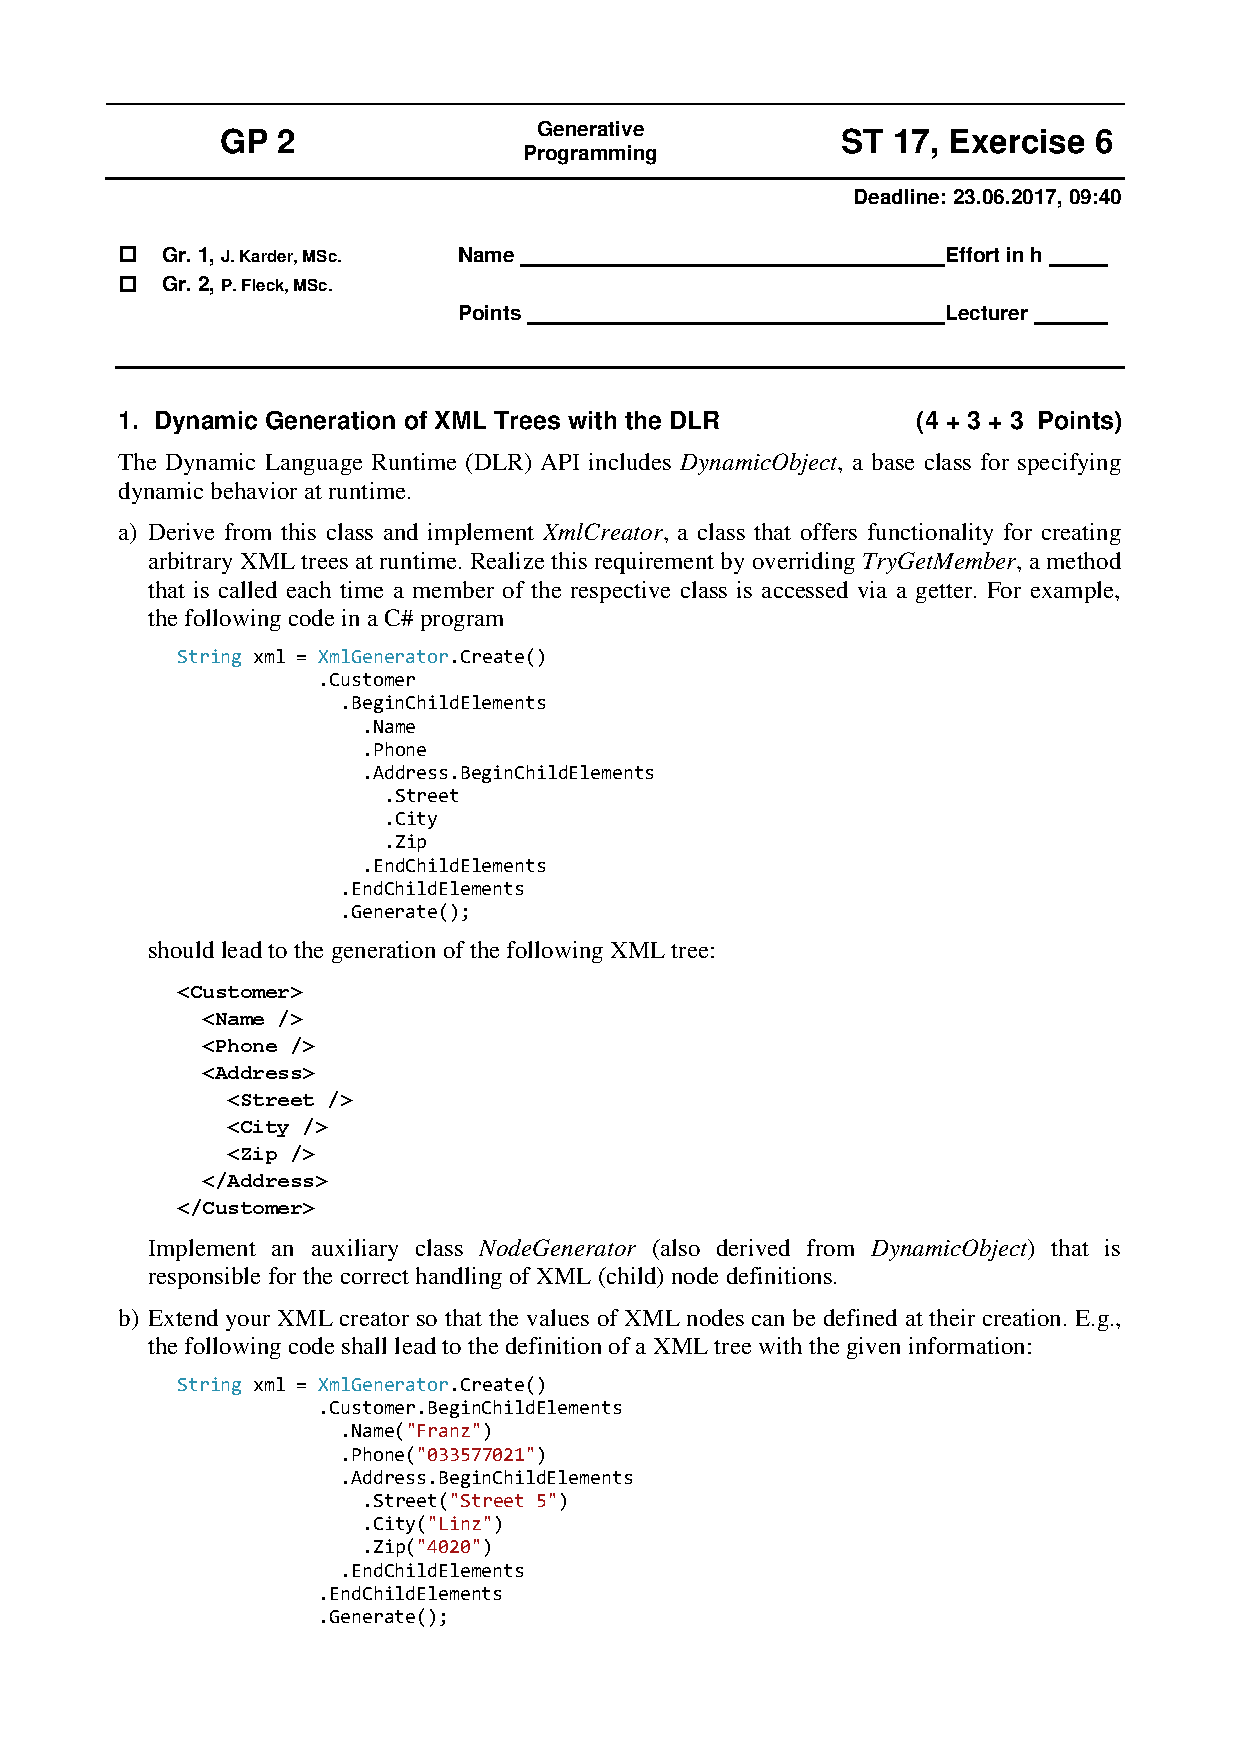
\includepdf[pages={1,2,3}]{GP_A06.pdf}

\section{\emph{Dynamic Generation of XML Trees with the DLR}}
Dieser Abschnitt behandelt die Aufgabenstellung \emph{Dynamic Generation of XML Trees with the DLR}.

\subsection{Lösungsidee} 
Es wird die Klasse \emph{DynamicNode} als Ableitung der Klasse \emph{DynamicObject} implementiert, welche die XML Zeichenkette für die aktuelle \emph{Node} generiert und die Generierung ebenfalls an seine Kind Knoten weiter delegiert, die wiederum ihre XML String Repräsentation generieren. Die generierte XML Zeichenkette wird mit einem \emph{StringBuilder} aufgebaut. Die Klasse erstellt für jeden neuen \emph{Member} einen Knoten als Objekt der Klasse \emph{DynacmicNode}. Bei einem Methodenaufruf wird ebenfalls ein Kind Knoten erstellt, wobei die Argumente als XML Attribute behandelt werden. Wenn mehr als 3 Argumente angegeben wurden wird eine Ausnahme ausgelöst.
\newline
\newline
Es wird die Klasse \emph{XmlGenerator} implementiert, die auch eine Ableitung der Klasse \emph{DynamicObject} ist und für den ersten \emph{Member}, den \emph{Rootknoten} als Objekt der Klasse \emph{DynamicNode} erstellt.  

\subsection{Quelltexte}
Dieser Abschnitt beinhaltet die implementierten Quelltexte und das Testprogramm.
\begin{code}
	\caption{XmlGenerator.cs}
	\cppSourceFile{\srcXMLGenerator/XmlGenerator.cs}
	\label{src:xml-generator}
\end{code}

\begin{code}
	\caption{DynamicNode.cs}
	\cppSourceFile{\srcXMLGenerator/DynamicNode.cs}
	\label{src:xml-dynamic-node}
\end{code}

\begin{code}
	\caption{Program.cs}
	\cppSourceFile{\srcXMLGenerator/Program.cs}
	\label{src:xml-program}
\end{code}
\ \newpage

\subsection{Tests}
Dieser Abschnitt behandelt die Tests in Form von Ausgaben der \emph{Logs}.
\begin{figure}[h]
	\centering
	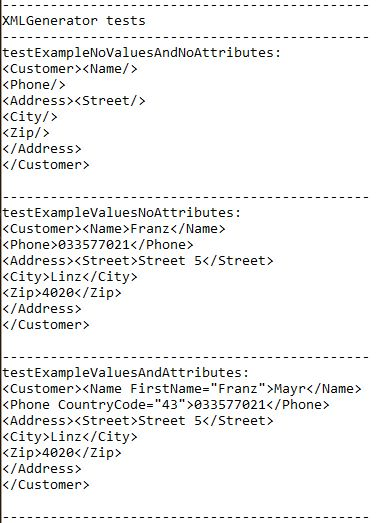
\includegraphics[scale=0.8]{\imageDir/test-xml-generator.JPG}
	\caption{Test für die XML Generierung}
	\label{fig:image-proxy-generator}
\end{figure}
\ \newpage

\section{\emph{Dynamic Generation of Proxies with the DLR}}
Dieser Abschnitt behandelt die Aufgabenstellung \emph{Dynamic Generation of Proxies with the DLR}.

\subsection{Lösungsidee}
Es wird die Klasse \emph{ProxyGenerator} implementiert, welche eine Ableitung der Klasse \emph{DynamicMetaObject} ist. Diese Klasse wird die Aspekte für das dynamische Objekt einweben, aber nur wenn ein Objekt der Schnittstelle \emph{IInterception} dieser Klasse übergeben wurde.
\newline
\newline
Es wird die Schnittstelle \emph{IInterception} implementiert, welche einen \emph{Interceptor} spezifiziert. Als Implementierung der Schnittstelle \emph{IInterception} wird die Klasse \emph{LogInterceptor} implementiert, die \emph{Properties} vom Datentyp \emph{bool} bereitstellt, mit denen das Ausführen der Methode und das Ersetzen des Resultats gesteuert werden kann. Ebenso wird ein \emph{Property} vom Datentyp \emph{object} bereitgestellt, mit dem das Resultat ersetzt werden soll, aber nur wenn der \emph{bool} \emph{Property} für das Ersetzen gesetzt wurde.
\newline
\newline
Es wird die Klasse \emph{DynamicTest} implementiert, welche eine Ableitung der Klasse \emph{IDynamicMetaObjectProvider} ist, wobei diese Implementierung das Metaobjekt erzeugt, das in ein Objekt der Klasse \emph{ProxyGenerator} ist.

\subsection{Quelltexte}
Dieser Abschnitt beinhaltet die implementierten Quelltexte und das Testprogramm.
\begin{code}
	\caption{IInterception.cs}
	\cppSourceFile{\srcProxyGenerator/IInterception.cs}
	\label{src:interception}
\end{code}

\begin{code}
	\caption{LogInterception.cs}
	\cppSourceFile{\srcProxyGenerator/LogInterception.cs}
	\label{src:log-interception}
\end{code}

\begin{code}
	\caption{ProxyGenerator.cs}
	\cppSourceFile{\srcProxyGenerator/ProxyGenerator.cs}
	\label{src:proxy-generator}
\end{code}

\begin{code}
	\caption{DynamicTest.cs}
	\cppSourceFile{\srcProxyGenerator/DynamicTest.cs}
	\label{src:dynamic-test}
\end{code}

\begin{code}
	\caption{Program.cs}
	\cppSourceFile{\srcProxyGenerator/Program.cs}
	\label{src:dynamic-test-program}
\end{code}
\ \newpage

\subsection{Tests}

Dieser Abschnitt behandelt die Tests in Form von Ausgaben der \emph{Logs}.
\begin{figure}[h]
	\centering
	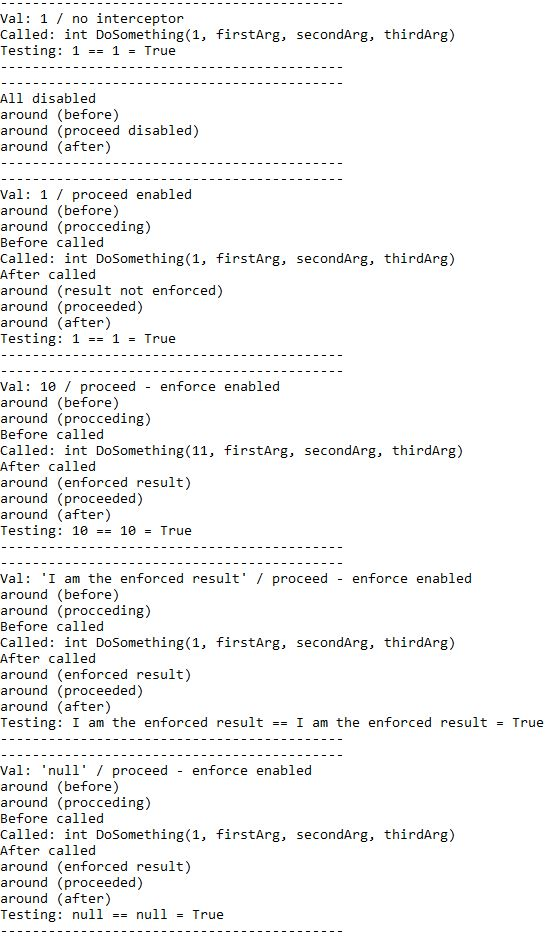
\includegraphics[scale=0.7]{\imageDir/test-proxy-generator.JPG}
	\caption{Test für die Proxy Generierung}
	\label{fig:image-test-proxy-generator}
\end{figure}

\end{document}